\documentclass[conference]{IEEEtran}
\IEEEoverridecommandlockouts
\usepackage{graphicx}
\usepackage{booktabs}
\usepackage{amsmath}
\usepackage[ruled,lined]{algorithm2e}

\usepackage{ifpdf}
\ifpdf
  \DeclareGraphicsExtensions{.pdf,.png}
\else
  \DeclareGraphicsExtensions{.eps}
\fi

%\IEEEoverridecommandlockouts                              % This command is only
%\overrideIEEEmargins


\title{Analysis traversability of  protein tunnels considering flexible ligands}

\author{
Barbora Kozl\'{i}kov\'{a}, Vojt\v{e}ch Von\'{a}sek, Martin Ma\v{n}\'{a}k
}

%Department of Cybernetics, Faculty of  Electrical Engineering\\ Czech Technical University in Prague
%Technicka 2, 166 27, Prague 6, Czech Republic.

\begin{document}

\maketitle

\begin{abstract}
TODO
\end{abstract}

\section{Introduction}

The van der Waals model of a protein is given by centers $\mathbf{c}_i \in R^3$ and radii $r_i \in R^+$ of individual atoms. An example with a ligand bound to the protein is depicted in \figurename~\ref{fig:vd}. Dynamic models add the movement of atoms by specifying positions in subsequent time-snapshots. In our research we develop methods for planning almost collision-avoiding paths for flexible ligands in dynamic protein models. We join computational geometry concepts, path-planning approaches and advanced visualization techniques to target this problem.

\section{Geometry}

The additively weighted Voronoi diagram (AWD) is a collection of regions $V\!R_i$ assigned to the corresponding atoms.
\[V\!R_i = \{x \in \mathbf{R}^3 \,:\,|\mathbf{x}-\mathbf{c}_i|-r_i \leq |\mathbf{x}-\mathbf{c_j}|-r_j\,\forall j \in I_n \}\]
Voronoi vertices and edges provide us a description of free space among atoms with respect to a spherical probe as it is depicted on a 2D analogy in \figurename~\ref{fig:vd}. Our program computes AWD for each time-snapshot of the dynamic model in a pre-processing phase and then offers this data to the motion-planning part. The rationale is that paths that are good for a single probe can also be good for a complex ligand.

\begin{figure}[htb]
\centering
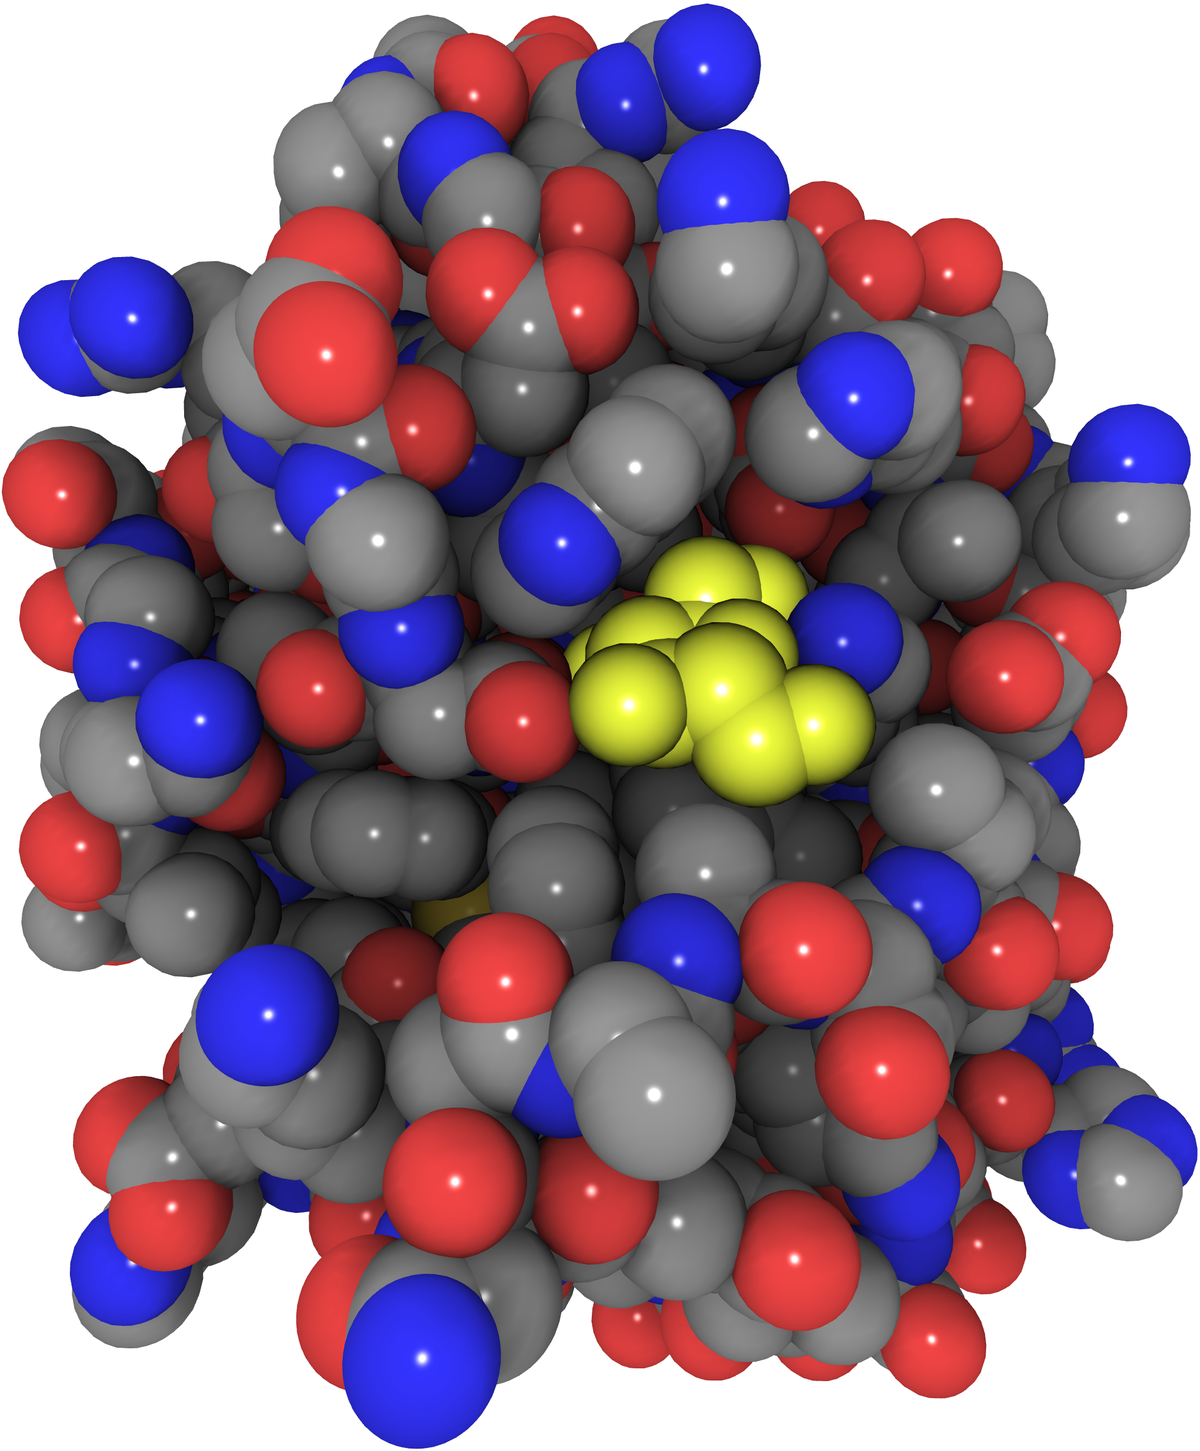
\includegraphics[height=10em]{figures/4b1m}
\hspace{1em}
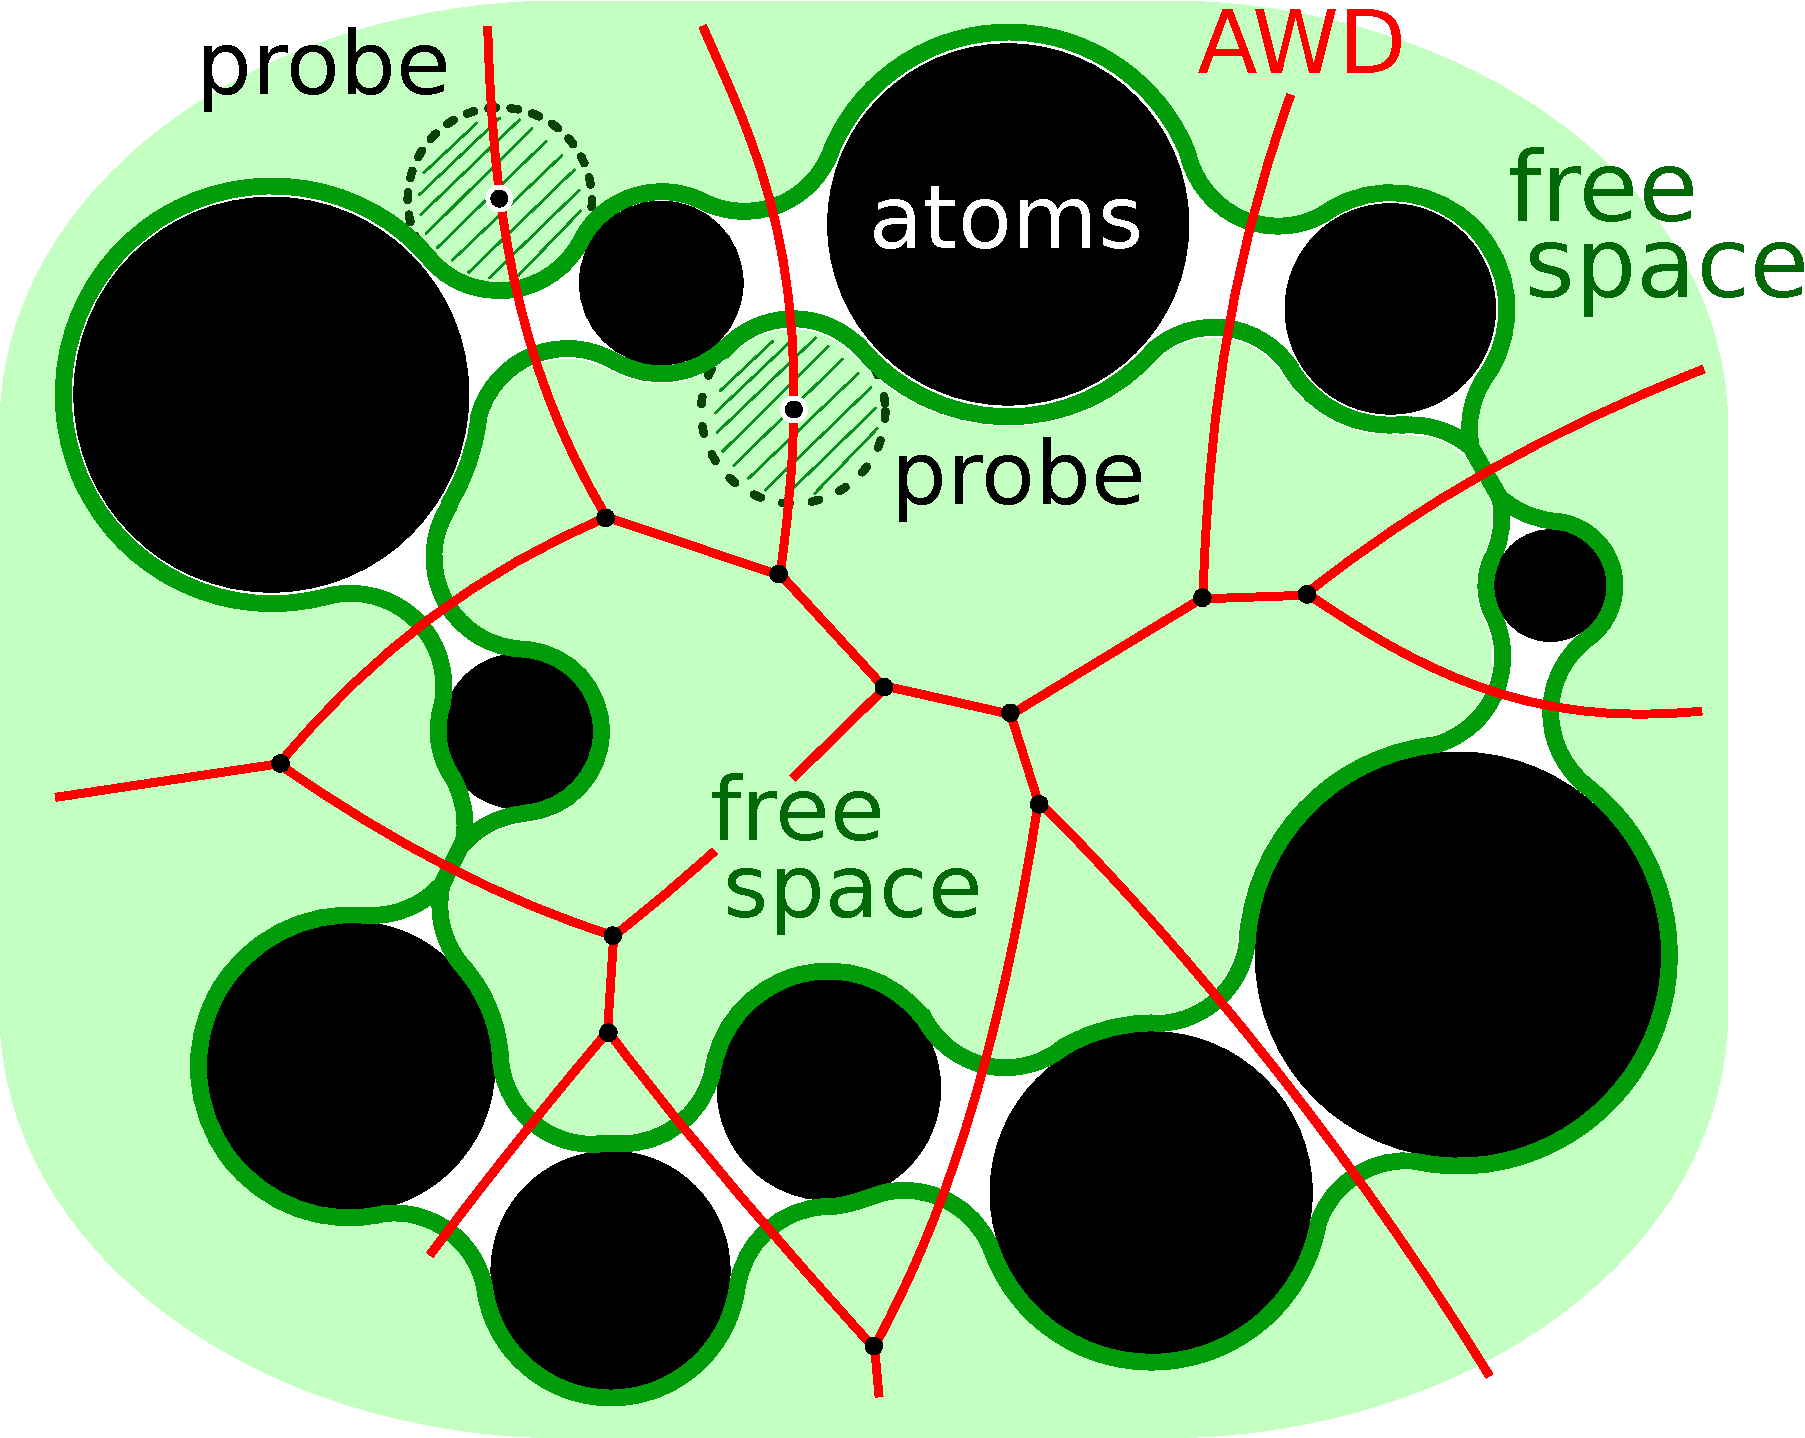
\includegraphics[height=10em]{figures/awd}
\caption{The protein 4B1M \cite{Cuskin2012} and its van der Waals model with a ligand; The~\mbox{aw-Voronoi} diagram for the analysis of free space by spherical probes}
\label{fig:vd}
\end{figure}

\section{Path-planning}

By searching paths in the constructed AWD, tunnels can be identified in the protein.
These tunnels however describe possible pathways for single atom.

To compute trajectories for non-spherical ligands, considering their shape and conformational changes, 
motion planning techniques, originally studied in the field of robotics, are applied.
The ligand is considered as a flexible robot moving among obstacles defined by the protein atoms.
It is necessary to consider ligand translation, rotation and also additional degrees of freedom defined by the flexible dihedral angles.
Finding of trajectories for such a system leads to a search in a high-dimensional configuration space, which can be efficiently
solved using sampling-based planners~\cite{Lav06}.

We utilize a modified Rapidly Exploring Random Tree Planner (RRT)~\cite{vonasek2017tunnel}, that builds
a tree of collision-free configurations of the ligand (a configuration defines position, translation and internal DOFs of the ligand).
Unlike classic RRT-based planners, that sample the space uniformly, we utilize the constructed AWD to sample the position
of the ligands near the vertices of the AWD.
This allows us to find trajectories along the tunnels and it is also faster than sampling the whole configuration space uniformly.
In each iteration, a random sample is generated around a vertex of AWD and its nearest node in the tree is found.
Then, the tree is expanded towards the random sample from the nearest node. 
During the expansion, collision-detection between the ligand and the protein is checked and the tree is expanded only by the 
collision-free nodes.
The method terminates if the tree reaches the desired goal state, which is  defined e.g. as the position of the active site.

The resulting trajectories are then evaluated using an energy function (using Vina Autodock tool~\cite{trott2009autodock}).


\section{Visualization}

\section*{Acknowledgments}
This work was supported by the project 17-07690S of the Czech Science Foundation.

%\includegraphics[width=0.2\textwidth]{fig/graphisbt}  
%\includegraphics[width=0.25\textwidth]{fig/graph3d} 

\bibliographystyle{abbrv}
\bibliography{poster}

\end{document}
